\documentclass[conference]{IEEEtran}

% ==== packages ====
\usepackage{amsmath,amssymb}
\usepackage{graphicx}
\usepackage{booktabs}
\usepackage{siunitx}
\usepackage{xcolor}
\usepackage[hidelinks]{hyperref}
\usepackage{placeins} % \FloatBarrier(図の先走り防止)
\usepackage{tikz}
\usetikzlibrary{calc,positioning,arrows.meta,shapes,fit}

% ---- TikZ styles ----
\tikzset{
  box/.style = {draw, rounded corners=2pt, align=center, minimum height=0.9cm, font=\normalsize},
  flowstep/.style = {box, minimum width=3.6cm}, % 以前の "step" を flowstep に改名
  small/.style = {font=\small},
  sum/.style = {circle, draw, inner sep=1pt, minimum size=4mm},
  block/.style = {draw, minimum width=1.6cm, minimum height=0.9cm, align=center},
  line/.style = {->, >=Stealth}
}

\begin{document}

\title{AITL on Space: A Robust Three-Layer Architecture\\
with a Tri-NVM Hierarchy (SRAM / MRAM / FRAM)\\
for Long-Duration Spacecraft Autonomy}

\author{Shinichi Samizo\\
Independent Semiconductor Researcher\\
Former Engineer at Seiko Epson Corporation\\
Email: shin3t72@gmail.com\quad GitHub: \url{https://github.com/Samizo-AITL}
}

\maketitle

% ------------------------------------------------------------
% Abstract(図はここより前に出ない)
% ------------------------------------------------------------
\begin{abstract}
We propose AITL on Space, a three-layer control architecture (Robust Core, FSM Supervisor, AI Adaptor) implemented on a 22\,nm FDSOI SoC with a hardened tri-NVM hierarchy (SRAM/MRAM/FRAM). The system targets ultra-robust autonomy under radiation, thermal cycling, and long-term drift. This paper outlines the architecture, an 11D state-space plant model (8--20D extensible), an $H_\infty$ mixed-sensitivity design flow, and a verification pipeline from FPGA HIL to ASIC.
\end{abstract}

% ------------------------------------------------------------
\section{Introduction}
Long-duration missions require high availability under total ionizing dose (TID), single-event effects (SEE), and thermal cycles. Conventional PID + Flash architectures hit reliability limits due to charge-trap drift and write endurance. We summarize related work and motivate AITL on Space as a resilient alternative.

% ------------------------------------------------------------
\section{System Architecture}
AITL comprises three layers:
\begin{itemize}
  \item \textbf{Robust Core} for $H_\infty$/MPC/SMC control,
  \item \textbf{FSM Supervisor} (Safe/Nominal/Recovery; FDI/FDII),
  \item \textbf{AI Adaptor} for long-term re-identification and drift compensation.
\end{itemize}
A tri-NVM hierarchy is adopted: \emph{SRAM} for execution, \emph{MRAM} for code/logs (ECC + scrub, A/B slots), and \emph{FRAM} for safe boot and FSM state. The target implementation is a 22\,nm FDSOI SoC hardened for radiation and temperature cycling.

% ---------------- Fig.1 ----------------
\begin{figure*}[t]
\centering
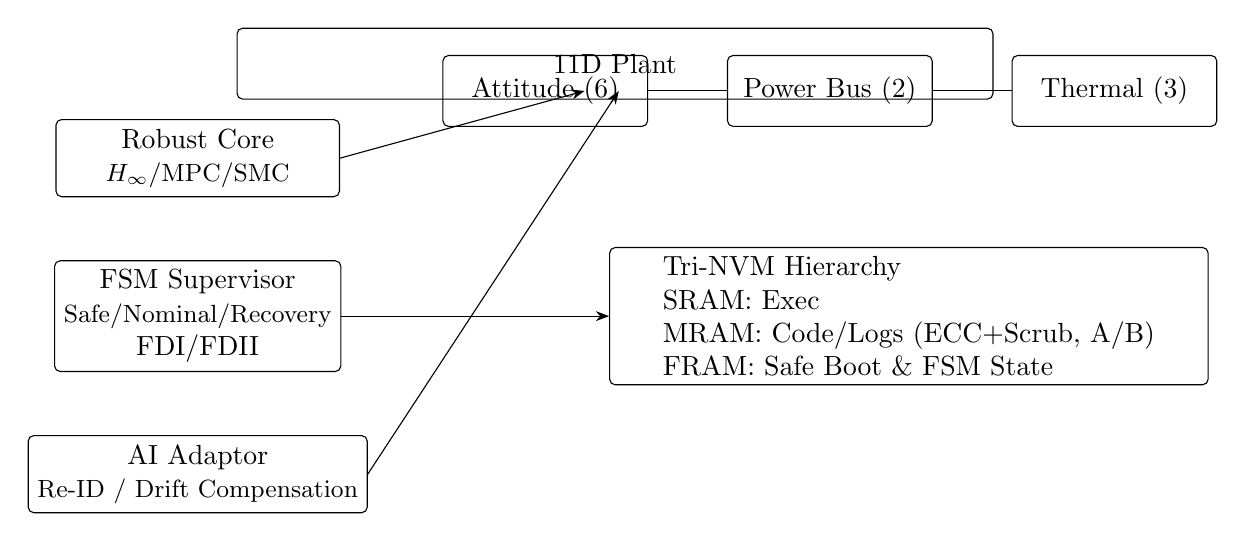
\begin{tikzpicture}[node distance=8mm and 10mm]
  % plant bus header
  \node[box, minimum width=9.6cm] (plant) {11D Plant};

  % left column boxes
  \node[box, below left=12mm and 23mm of plant.west, anchor=west, minimum width=3.6cm]
        (robust) {Robust Core\\\small $H_\infty$/MPC/SMC};
  \node[box, below=8mm of robust, minimum width=3.6cm]
        (fsm) {FSM Supervisor\\\small Safe/Nominal/Recovery\\FDI/FDII};
  \node[box, below=8mm of fsm, minimum width=3.6cm]
        (ai) {AI Adaptor\\\small Re-ID / Drift Compensation};

  % right column tri-NVM box
  \node[box, right=34mm of fsm, anchor=west, minimum width=7.6cm, align=left]
        (nvm) {Tri-NVM Hierarchy\\
        SRAM: Exec\\
        MRAM: Code/Logs (ECC+Scrub, A/B)\\
        FRAM: Safe Boot \& FSM State};

  % plant internal boxes
  \node[box, above right=-1mm and 13mm of robust.north east, minimum width=2.6cm] (att) {Attitude (6)};
  \node[box, right=10mm of att, minimum width=2.6cm] (bus) {Power Bus (2)};
  \node[box, right=10mm of bus, minimum width=2.6cm] (therm) {Thermal (3)};

  % connections
  \draw[line] (robust.east) -- ($(att.west)!0.5!(bus.west)$);
  \draw[line] (fsm.east) -- (nvm.west);
  \draw[line] (ai.east)  -- ($(att.west)!0.62!(bus.west)$);
  \draw (att) -- (bus) -- (therm);
\end{tikzpicture}
\caption{AITL on Space architecture with Robust Core, Supervisor FSM, AI Adaptor, and the Tri-NVM hierarchy.}
\label{fig:arch}
\end{figure*}

% ------------------------------------------------------------
\section{Mathematical Model}
We use an 11D discrete-time plant that couples attitude (6), power bus (2), and thermal nodes (3):
\begin{align}
x_{k+1} &= A x_k + B u_k + E w_k, \label{eq:ss1}\\
y_k &= C x_k + D u_k + v_k. \label{eq:ss2}
\end{align}
The model extends to 20D by adding translational axes and bias states. $w_k$ and $v_k$ represent disturbance and sensor noise, respectively.

% ---------------- Fig.2 ----------------
\begin{figure}[t]
\centering
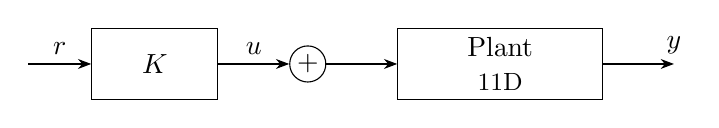
\begin{tikzpicture}
  \node[block] (K) {$K$};
  \node[sum, right=9mm of K] (sum) {$+$};
  \node[block, right=9mm of sum, minimum width=2.6cm] (P) {Plant\\\small 11D};
  \draw[line] ($(K.west)+(-8mm,0)$) -- (K.west) node[midway, above] {$r$};
  \draw[line] (K) -- node[above] {$u$} (sum);
  \draw[line] (sum) -- (P);
  \draw[line] (P.east) -- ++(9mm,0) node[above] {$y$};
\end{tikzpicture}
\caption{Closed-loop schematic used for $H_\infty$ synthesis on the 11D plant.}
\label{fig:loop}
\end{figure}

% ------------------------------------------------------------
\section{$H_\infty$ Mixed-Sensitivity Design}
Weights $(W_1,W_2,W_3)$ shape sensitivity, control effort, and complementary sensitivity, respectively. \emph{EduController} exports JSON plant/weights; \emph{AITL-H} synthesizes an output-feedback $K$ and a fixed-point realization suitable for FPGA/ASIC.

% ------------------------------------------------------------
\section{Verification Pipeline}
FPGA HIL injects SEU bursts and sensor outages. Metrics include safe-mode time ($<\!1$\,s), recovery rate ($\ge\!99\%$), and ECC statistics under scrubbing. Physical design proceeds to 22FDX tape-out; \emph{SystemDK} FEM closes thermal/packaging with radiation/temperature scenarios.

% ---------------- Fig.3 ----------------
\begin{figure}[t]
\centering
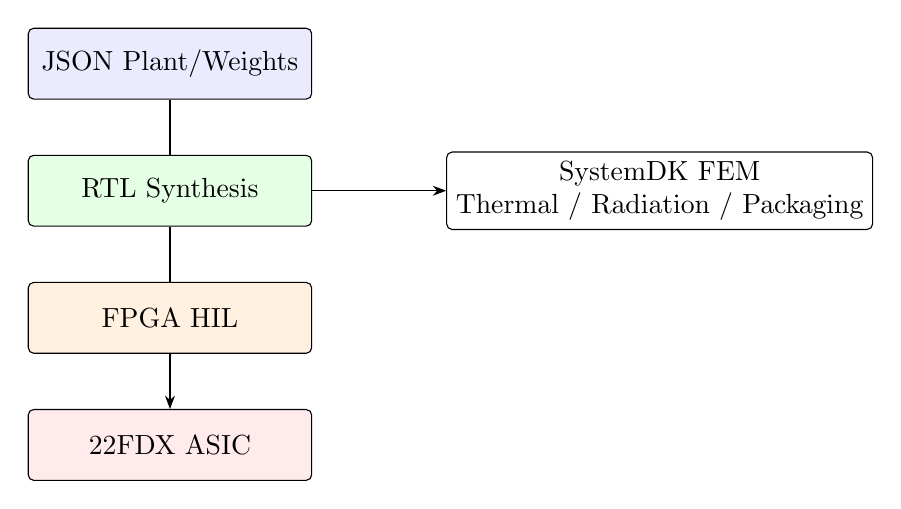
\begin{tikzpicture}[node distance=7mm]
  \node[flowstep, fill=blue!8] (json) {JSON Plant/Weights};
  \node[flowstep, fill=green!10, below=of json] (rtl) {RTL Synthesis};
  \node[flowstep, fill=orange!12, below=of rtl] (hil) {FPGA HIL};
  \node[flowstep, fill=red!8, below=of hil] (asic) {22FDX ASIC};
  \node[box, right=17mm of rtl, minimum width=4.8cm, align=center] (fem)
        {SystemDK FEM\\Thermal / Radiation / Packaging};
  \draw[line] (json) -- (rtl) -- (hil) -- (asic);
  \draw[line] (rtl) -- (fem);
\end{tikzpicture}
\caption{Verification pipeline from JSON design to RTL, FPGA HIL, and ASIC; FEM closes the loop with thermal and radiation scenarios.}
\label{fig:pipeline}
\end{figure}

% ------------------------------------------------------------
\section{Conclusion}
AITL on Space provides a practical path to resilient autonomy for deep-space missions by combining robust control, supervisory safety logic, AI-based re-identification, and a tri-NVM memory hierarchy.

% ------------------------------------------------------------
\section*{References}
\begin{thebibliography}{99}
\bibitem{doyle}
J.\,C.~Doyle, B.\,A.~Francis, and A.\,R.~Tannenbaum, \emph{Feedback Control Theory}. Macmillan, 1992.
\bibitem{colinge}
J.-P.~Colinge, \emph{Silicon-on-Insulator Technology: Materials to VLSI}, 3rd ed. Springer, 2004.
\end{thebibliography}

% ------------------------------------------------------------
\section*{Author Biography}
Shinichi Samizo received the M.S. degree in Electrical and Electronic Engineering from Shinshu University, Japan. He worked at Seiko Epson Corporation as an engineer in semiconductor memory and mixed-signal device development, and contributed to inkjet MEMS actuators and PrecisionCore printhead technology. He is currently an independent semiconductor researcher focusing on process/device education, memory architecture, and AI system integration. Contact: \texttt{shin3t72@gmail.com}.

\FloatBarrier % 図が巻き戻って Abstract より前に出ないように固定

\end{document}
